%%%%%%%%%%%%%%%%%%%%%%%%%%%%%%%%%%%%%%%%%%%%%%%%%%%%%%%%%%%%%%%%%%%%%%%%%%%%%%%%
%2345678901234567890123456789012345678901234567890123456789012345678901234567890
%        1         2         3         4         5         6         7         8

\documentclass[letterpaper, 10 pt, conference]{ieeeconf}  % Comment this line out
                                                          % if you need a4paper
%\documentclass[a4paper, 10pt, conference]{ieeeconf}      % Use this line for a4
                                                          % paper
\usepackage[english]{babel}
\usepackage[utf8]{inputenc}
\usepackage{amsmath}
\usepackage{blindtext}
\usepackage{scrextend}
\usepackage{fontawesome5}
\usepackage{graphicx}
\usepackage{hyperref}
\usepackage{upgreek}
\usepackage{listings}
\usepackage[export]{adjustbox}
\usepackage[colorinlistoftodos]{todonotes}
\IEEEoverridecommandlockouts                              
\overrideIEEEmargins

\definecolor{codegreen}{rgb}{0,0.6,0}
\definecolor{codegray}{rgb}{0.5,0.5,0.5}
\definecolor{codepurple}{rgb}{0.58,0,0.82}
\definecolor{backcolour}{rgb}{0.95,0.95,0.92}

\lstdefinestyle{mystyle}{
    backgroundcolor=\color{backcolour},   
    commentstyle=\color{codegreen},
    keywordstyle=\color{magenta},
    numberstyle=\tiny\color{codegray},
    stringstyle=\color{codepurple},
    basicstyle=\ttfamily\footnotesize,
    breakatwhitespace=false,         
    breaklines=true,                 
    captionpos=b,                    
    keepspaces=true,                 
    numbers=left,                    
    numbersep=5pt,                  
    showspaces=false,                
    showstringspaces=false,
    showtabs=false,                  
    tabsize=2
}

\lstset{style=mystyle}

\title{\LARGE \bf
ZKU – Cohort 4 (Jul-Aug 2022)\\Week 1: Introduction to ZKP\\Assignment \sharp 1}

% \author{Iskander Andrews\\\faIcon{discord} Isk#0996}
\author{Iskander Andrews$^{1}$% <-this % stops a space
\thanks{\faIcon[regular]{envelope} \tt\small iskander.s.andrews@gmail.com}
\thanks{\faIcon{discord} \tt\small Isk#0996}
\thanks{\faIcon{github} \tt\small iskdrews}}

\begin{document}



\maketitle
\thispagestyle{empty}
\pagestyle{empty}


%%%%%%%%%%%%%%%%%%%%%%%%%%%%%%%%%%%%%%%%%%%%%%%%%%%%%%%%%%%%%%%%%%%%%%%%%%%%%%%%
\begin{abstract}

This document is for answering ZKUC04, Week-1, Introduction to ZKP Assignment.
It consists of three main parts.
\begin{labeling}{alligator}
\item [\textbf{Part 1:}] Theoretical background of zk-SNARKs and zk-STARKS.
\item [\textbf{Part 2:}] Getting started with circom and snarkjs.
\item [\textbf{Part 3:}] Reading and designing circuits with Circom.
\end{labeling}

The total number of questions and points is $13$, including the bonus questions. 
\end{abstract}

\noindent\rule{8cm}{0.4pt}

\section{\textbf{\underline{Part 1:}} Theoretical background of zk-SNARKs and zk-STARKS}
\subsection{\textbf{\underline{1.1} Explain in 2-4 sentences why SNARK requires a trusted setup while STARK doesn’t.}}

zkSTARKs requires a trusted setup because it requires an initial creation event of the keys, which are used to create proofs for private transactions, and used in the verification of those proofs. \newline On the other hand, zkSTARKs does not require a trusted-setup for utilizing the network because it is transparent which means that they use publicly verifiable randomness to create a trustless verifiable computing system. \cite{c1}\cite{c2}

\subsection{\textbf{\underline{1.2} Name two more differences between SNARK and STARK proofs.}}
\begin{enumerate}
  \item zkSTARKs rely on hash functions, so it would be a quantum resistant, on the other hand zkSNARKs are not quantum resistant so the privacy of SNARKs could be broken. \cite{c1}
  \item zkSTARKs have larger proof sizes than zkSNARKs, which means that the verification in STARKs takes more time than in SNARKs. \cite{c1}
\end{enumerate}

\noindent\rule{8cm}{0.4pt}

\section{\textbf{\underline{Part 2:}} Getting started with circom and snarkjs:}
\subsection{\textbf{\underline{Question (1)}}}
\subsubsection{\textbf{\underline{2.1} What does the circuit in HelloWorld.circom do?}}

It implements a Circom circuit to prove the multiplication of two private inputs signal identifiers a, and b,and calculate the result in a public output signal identifier c. 

\subsection{\textbf{\underline{Question (2)}}}
\subsubsection{\textbf{\underline{2.2.1} What is a Powers of Tau ceremony?}}

The Power of Tau ($\tau$) is a secure multi-party computation (\textit{MPC}) ceremony. It is used in generating the parameters of the first phase (1) in zkSNARK which consists of two phases. It can generate paramters for all the circuits up to a depth of $2^{21}$. 
It proceeds in turns, one turn for each party, and the result of the computation of each party is then added to a public transcript, which will allow all the system be verified. The result parameters of the system then becomes secure if one party was able to destroy the random toxic waste. \cite{c3}

\subsubsection{\textbf{\underline{2.2.2} Explain why this is important in the setup of zk-SNARK applications.}}


In order to deploy a zkSNARK circuits, a developer must perform a computation for generating the "Proving Key", and the "Verifying key", and this process called a "Trusted Setup". There is a downside for this process because it produces bad numbers called "toxic waste" file that needs to be destroyed otherwise it will produce fake proofs which will violate the security of the system. So to resolve that, the "Trusted Setup" can be setup using specific Cryptographic ceremony like the "Powers of Tau" ceremony, which will be used only in generating the first phase of parameter generation of all the projects, since zk-SNARKs requires two phases of parameter generation. \cite{c4}

Power of Tau ceremony is helping in creating what is called a "Chain of trusted-setup", through allowing multiple parties to setup a trusted setup and then adding the results to a public transcript, and the system can be verified by publishing the results. Moreover, the system will be considered secure, if only one of the parties has successfully destroying the "toxic waste" file. \cite{c5}

\subsubsection{\textbf{\underline{2.2.3} How are Phase 1 and Phase 2 trusted setup ceremonies different from each other?}}

zkSNARK projects consists of two phases of parameter generation, The Power of Tau can be only used in the first phase for all the projects. While the second phase if a circuit-speicfic that needs to be done for each circuit, and the individual teams are responsible on it. 
\newline Phase-one is a universal phase ceremony for the entire community, while to start phase-two, any zkSNARK projects can pick any point of the ceremony to begin their circuit-specific second phase. \cite{c4} \cite{c6}

\begin{figure}[htp]
    \centering
    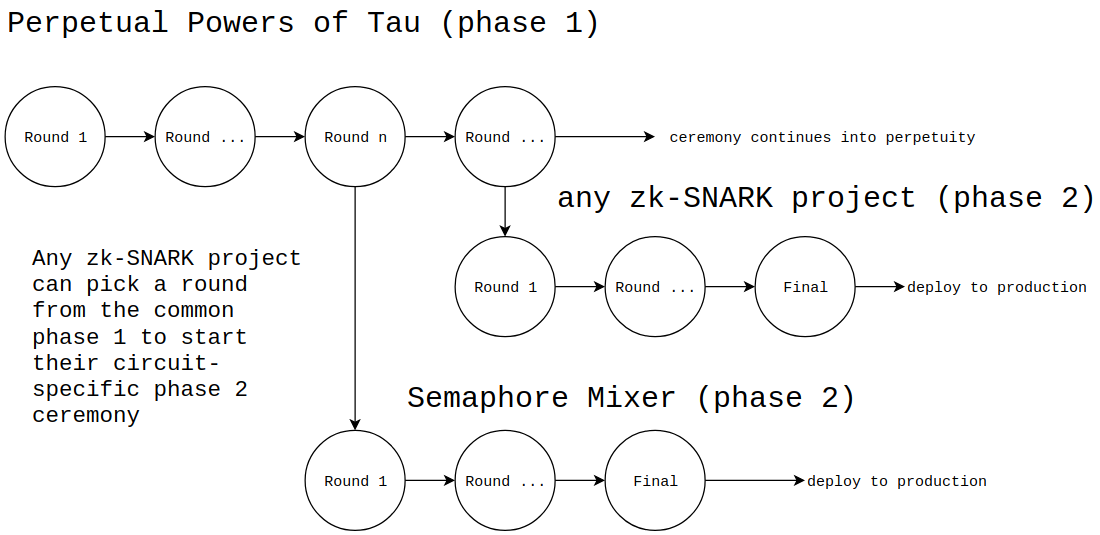
\includegraphics[width=9cm]{assets/phase1-phase2}
    \caption{Image borrowed from Wei Jie Koh’s post. \cite{c4}}
    \label{fig:galaxy}
\end{figure}

\subsection{\textbf{\underline{Question (3)}}}

\subsubsection{\textbf{\underline{2.3.2} Try to run \textcolor{red}{\textit{compile-Multiplier3-groth16.sh}}. You should encounter an \textcolor{red}{\textit{error[T3001]}} with the circuit as is. Explain what the error means and how it arises.}}

\textcolor{red}{\textit{error[T3001]}} means that the constraint is Non-quadratic expression, because it should be one of those constraints: \cite{c7}

\begin{labeling}{alligator}
\item [\textbf{Constant values}] 
\item [\textbf{Linear expression}]    $2*x + 3*y + 2$
\item [\textbf{Quadratic expression}] $(2*x + 3*y + 2) * (x+y) + 6*x + y – 2$ 
\end{labeling}  

\subsection{\textbf{\underline{Question (4)}}}
\subsubsection{\textbf{\underline{2.4.1} What are the practical differences between Groth16 and PLONK? Hint: compare and contrast the resulted contracts and running time of unit tests from the two protocols. }}



\subsection{\textbf{\underline{Question (5)}}}
\subsubsection{\textbf{\underline{2.5.3} In \textcolor{red}{test/test.js}, add the unit tests for \textcolor{red}{Multiplier3} for both the Groth16 and PLONK versions. Include a screenshot of all the tests (for \textcolor{red}{HelloWorld, Multiplier3 with Groth16}, and \textcolor{red}{Multiplier3 with PLONK}) passing in your PDF file.}}

\begin{figure}[htp]
    \centering
    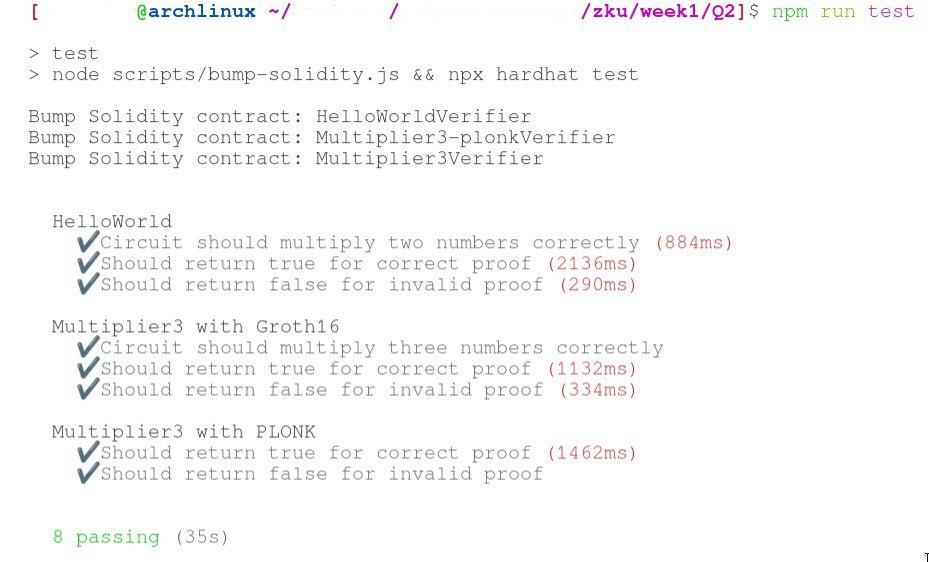
\includegraphics[width=9cm]{assets/photo_2022-07-11_08-53-09}
    \caption{All tests are passing.}
    \label{fig:galaxy}
\end{figure}

\noindent\rule{8cm}{0.4pt}




\section{\textbf{\underline{Part 3:}} Reading and designing circuits with Circom}

\subsection{\textbf{}\underline{Question (1)}}
\subsubsection{\textbf{\underline{3.1.1} What does the $32$ in Line $9$ stand for?}}

$n$ variable in the \textcolor{red}{template LessThan(n)} function refers to the number of bits for the input signal, and $32$ stands for the unsigned integers, non-negative integer in the range $[0 to 4294967295]$.

\subsubsection{\textbf{\underline{3.1.2} What are the possible outputs for the LessThan template and what do they mean respectively?}}

The expected outputs are either $0$ or $1$ which is a boolean return datatype, so if the number $n1$ is not less than number $n2$ the output will be $0$ which means false $n1 > n2$. Otherwise the output will be $1$ which means true $n1 < n2$.

\subsection{\textbf{\underline{Question (2)}}}

\subsubsection{\textbf{\underline{3.2.2} You can run \textcolor{red}{npm run test:fullProof} while inside the \textcolor{red}{zkPuzzles} directory to test your modified circuit. You are expected to encounter an error. Record the error, resolve it by modifying \textcolor{red}{project/zkPuzzles/scripts/compile-circuits.sh}, and explain why it has occurred and what you did to solve the error?}}

The error was \textcolor{red}{[ERROR] snarkJS: circuit too big for this power of tau ceremony. $97588 > 2^{16}$}.
It means that the current circuit requires a bigger power of tau ceremony, because the current one is a $16$ ceremony $2^{16} < 97588$, which is less than the expected from the circuit $97588$. To resolve this error, just change the downloaded Power of Tau ceremony file to be bigger than $16$, so I downloaded Power of Tau with the power of $20$ therefore, $2^{20} > 97588$.

\begin{lstlisting}[language=Bash, caption=Expected solution]
# ./zku/week1/Q3/projects/zkPuzzles/scripts
if [ -f ./powersOfTau28_hez_final_20.ptau ]; then
    echo "powersOfTau28_hez_final_20.ptau already exists. Skipping."
else
    echo 'Downloading powersOfTau28_hez_final_20.ptau'
    wget https://hermez.s3-eu-west-1.amazonaws.com/powersOfTau28_hez_final_20.ptau
fi
\end{lstlisting}

\subsection{\textbf{\underline{Question (4) [Bonus]}}}
\subsubsection{\textbf{\underline{3.4} what other libraries do you think could be created to help foster the growth of ZK applications?}}

I think it would be better if there is a support for strings in the debugging log() library, that would be useful to separate between the printed logs, for exmaple: \textcolor{red}{log("Single input in",  in);}.
Also, it would be useful if there are a static typing system for the templates and the functions, typing the data-types of the expected inputs and the expected return.

\noindent\rule{8cm}{0.4pt}

\section*{ACKNOWLEDGMENT}
The preferred spelling of the word ÒacknowledgmentÓ in America is without an ÒeÓ after the ÒgÓ. Avoid the stilted expression, ÒOne of us (R. B. G.) thanks . . .Ó  Instead, try ÒR. B. G. thanksÓ. Put sponsor acknowledgments in the unnumbered footnote on the first page.

\noindent\rule{8cm}{0.4pt}
\begin{thebibliography}{99}

\bibitem{c1} Mattison Asher, Coogan Brennan, Zero-Knowledge Proofs: STARKs vs SNARKs, May 18, 2021. \href{https://consensys.net/blog/blockchain-explained/zero-knowledge-proofs-starks-vs-snarks/}{\underline{link}}
\bibitem{c2} EthHub, ZK-STARKs. \href{https://docs.ethhub.io/ethereum-roadmap/layer-2-scaling/zk-starks/}{\underline{link}}
\bibitem{c3} github.com/ebfull/powersoftau. \href{https://github.com/ebfull/powersoftau}{\underline{link}}
\bibitem{c4} Koh Wei Jie, Announcing the Perpetual Powers of Tau Ceremony to benefit all zk-SNARK projects, Sep 11, 2019. \href{https://medium.com/coinmonks/announcing-the-perpetual-powers-of-tau-ceremony-to-benefit-all-zk-snark-projects-c3da86af8377#:~:text=The%20Powers%20of%20Tau%20ceremony,protocol%20can%20be%20publicly%20verified.&text=Nevertheless%2C%20each%20ceremony%20takes%20time%20and%20is%20tedious%20to%20coordinate.}{\underline{link}}
\bibitem{c5} Polygon Hermez, Hermez Zero-Knowledge Proofs, 2020. \href{https://blog.hermez.io/hermez-zero-knowledge-proofs/}{\underline{link}}
\bibitem{c6} Matthew Finestone, Loopring Begins zkSNARK Trusted Setup Multi-Party Computation Ceremony, Nov 10, 2019 \href{https://medium.com/coinmonks/loopring-starts-zksnark-trusted-setup-multi-party-computation-ceremony-cd1b98113773#:~:text=There%20are%20two%20phases%20for,circuit%20in%20the%20Loopring%20protocol.}{\underline{link}}
\bibitem{c7} Circom official documentations. \href{https://docs.circom.io/circom-language/constraint-generation/}{\underline{link}}
\end{thebibliography}

\end{document}
